\documentclass[12pt]{article}

\usepackage{fullpage}
\usepackage{graphicx, rotating, booktabs} 
\usepackage{times} 
\usepackage{natbib} 
\usepackage{indentfirst} 
\usepackage{setspace}
\usepackage{grffile} 
\usepackage{hyperref}
\usepackage{adjustbox}
\usepackage{amsmath}
\usepackage{siunitx}
\usepackage{multirow}
\setcitestyle{aysep{}}


\singlespace
\title{\textbf{Democracy, Elections, and Alliance Treaty Depth}}
\author{Joshua Alley \\
Postdoctoral Research Associate \\
University of Virginia\thanks{Thanks to Jasen Castillo, William Roberts Clark, Matthew Fuhrmann, Hyeran Jo and Todd Sechser for helpful comments.} 
}
\date{\today}

\bibliographystyle{apsr}

\begin{document}

\maketitle 

\doublespace 

\begin{abstract}
Why do states form deep alliance treaties, which reinforce military support promises with commitments of defense coordination and cooperation? 
I argue that democratic alliance leaders use treaty depth to make more credible alliance commitments even as leaders and ruling coalitions change. 
Elections can replace incumbents with new leaders who are less committed to an alliance. 
Such leadership turnover threatens credible alliance commitments by democracies, so incumbent leaders use treaty depth to make it more difficult and costly for future leaders to reduce alliance commitment. 
I test this claim on offensive and defensive alliances from 1816 to 2012 and illustrate the theoretical mechanisms by examining NATO.
I find that greater electoral democracy in the most capable alliance member increases treaty depth. 
The argument and findings provide insight into the connection between domestic politics and international institution design. 
\end{abstract}


\newpage 


\section{Introduction}


% Start with question and motive 
Why do states make deep alliance treaties? 
Deep alliances formalize extensive defense cooperation by using additional policy coordination and cooperation to supplement promises of military intervention. 
While shallow alliances offer arms-length military support, deep treaties lead to closer ties between alliance members. 
Key sources of depth include an integrated military command, military aid, defense policy coordination, basing rights, international organizations, and companion military agreements.
Half of all alliances that promise active military support include at least one such obligation \citep{Leedsetal2002}. 
Despite the prevalence of alliance treaty depth, why states add depth to their alliances is not well understood. 


% Generalize: IO design is not just primary commitments, but how states support/implement their promises
Understanding the rationale behind deep alliances is worthwhile for two reasons.
First, depth shapes alliance credibility and the distribution of military spending among alliance members. 
Costly commitments in deep alliances make military support promises more credible \citep{Morrow1994}, which then encourages non-major power members of deep alliances to reduce military spending \citep{Alley2020}.  
Second, other international institutions use costly commitments to support cooperation, so understanding the sources of treaty depth may provide more general insights into the design of international institutions.  
For example, some trade agreements use third-party dispute settlement mechanisms to enforce agreements \citep{Smith2000}, or institutionalize formal monitoring arrangements \citep{Duretal2013}.  
Understanding when and why states employ close or arms-length cooperative commitments is therefore worthwhile. 


% Describe question and contribution of the paper
In this paper, I argue that democratic alliance leaders use treaty depth to make more credible and durable alliance commitments. 
Depth helps leaders lock in alliance commitments in the face of leadership turnover and domestic political change. 
Although the leader negotiating an alliance is likely committed to upholding their treaty obligations, elections could empower less committed leaders and threaten alliance commitments \citep{GartzkeGleditsch2004, LeedsSavun2007, Leedsetal2009}.
In anticipation of this turnover threat, incumbent leaders employ treaty depth so their successors can signal commitment and undoing an alliance is more difficult and costly. 
Therefore, electoral democracy in the most capable alliance member encourages deep alliance treaties. 


% describe the test
I test the argument with a statistical analysis of offensive and defensive alliances from 1816 to 2018 and examine the theoretical mechanisms during NATO negotiations.
In my analysis, I disaggregate democratic institutions into electoral democracy and executive constraints, as my argument identifies electoral politics as the key source of treaty depth, and constraints could limit depth. 
I find consistent evidence that greater electoral democracy in the alliance leader increases treaty depth. 
The results are robust to different model specifications and samples, including a model that accounts for non-random selection into alliances. 


% Two Paras on the gap I fill 
This paper contributes to knowledge of alliance treaty design and how domestic politics affects alliances.
The process of alliance treaty negotiation and design is understudied in general \citep{Poast2019a}, and there is little research on depth because the nascent treaty design literature emphasizes conditions on military support \citep{Kim2011, Benson2012, Mattes2012, Chibaetal2015, FjelstulReiter2019}.
One set of arguments links democratic alliance membership with conditional treaty obligations through audience costs \citep{Mattes2012, Chibaetal2015, FjelstulReiter2019}. 
I differentiate the lock in process from a pure audience costs argument by examining the association between prior changes in the ruling coalition and treaty depth. 
The leadership turnover argument thus adds a new mechanism to the treaty design literature, isolates crucial characteristics of democracies, and contributes to the extensive literature on democracy and alliance politics e.g. \citep{LaiReiter2000, Mattes2012a, McManusYarhi-Milo2017}. 


Two previous studies have examined similar concepts to treaty depth \citep{Mattes2012, BensonClinton2016}. 
My analysis advances knowledge relative to this foundational work in two ways.  
First, my argument supplements the finding that symmetric bilateral alliances where one partner's leader had previously violated alliance obligations are more likely to use military institutionalization \citep{Mattes2012} and the analysis provides additional evidence from multilateral alliances.  
Second, while checking the validity of a latent measure of costly alliance obligations, \citet{BensonClinton2016} find that foreign policy agreement, major power involvement and treaty scope increase depth. 
Benson and Clinton define depth as how costly alliance obligations are in general, so their latent measure of depth includes secrecy and issue linkages.
My analysis focuses on costly defense cooperation, and explains why states might employ such cooperation. 


% implications: 
There are two primary implications of my argument and findings. 
To start, they add important nuance to existing claims that democracies prefer limited alliance commitments, especially conditional military support \citep{Mattes2012, Chibaetal2015, FjelstulReiter2019}.
My results suggest that regular leadership turnover pushes democracies to make more costly alliance commitments in other dimensions besides conditions on military support. 


Furthermore, I add to the rich literature on how domestic politics shapes international cooperation e.g. \citep{DownesRocke1995, Fearon1998, Leeds1999, MattesRodriguez2014}.
My argument explains how leaders strategically employ different foreign policy tools to strengthen international commitments within their domestic institutional context \citep{HydeSaunders2020}.  
Democracies' tendency to manage leadership turnover with deep alliances could apply to other international institutions. 
Just as democracies reassure partners with deep alliance commitments, electoral politics may push democracies to undertake deep international commitments.%\footnote{For example, in environmental agreements, democracies prefer soft law commitments \citep{BoehmeltButkute2018}, but other aspects of these agreements may be deep.} 


% roadmap for the paper 
%The paper proceeds as follows. 
%In the next section, I lay out the argument and hypotheses. 
%Then I summarize the data and research design. 
%After this, I describe the results and detail treaty depth considerations in NATO negotiations.
%In the final section I summarize the results and offer concluding thoughts. 


\section{Argument}


My argument starts by establishing the role of domestic politics in alliance negotiations. 
I then explain how leadership turnover in alliances threatens credible commitment. 
Last, I consider how depth addresses credibility concerns from regular leadership turnover. 


% explain allliances
Alliances are self-enforcing contracts or institutions where states promise military intervention \citep{Leedsetal2002, Morrow2000}. 
When faced with external threats in an anarchic international system, states form alliances to aggregate military capability and secure their foreign policy interests \citep{Snyder1997, FordhamPoast2014}.
Alliance participation has several costs and benefits.
Beyond the benefit of possible military support, alliances also clarify international alignments \citep{Snyder1997} and support economic ties \citep{Gowa1995, Long2003, Fordham2010, WolfordKim2017}.  
The costs of alliance participation include opportunism and lost foreign policy autonomy \citep{Altfield1984, Morrow2000, Johnson2015}. 
Opportunism in alliances has three forms; abandonment of military intervention promises \citep{BerkemeierFuhrmann2018}, entrapment in unwanted conflicts \citep{Snyder1984}, and free-riding \citep{Morrow2000}.


% process of alliance negotiations: establishing a credible commitment. 
To form an alliance, states must have similar foreign policy interests \citep{Morrow1991, Smith1995, FordhamPoast2014}. 
\citet{Poast2019a} notes that agreement over a treaty in alliance negotiations depends on outside options and compatible war plans. 
Alliance treaties formalizing promises of military support take many forms \citep{Leedsetal2002, BensonClinton2016}. 
Treaty design shapes the costs and benefits of treaty participation and addresses potential opportunism.  
In the face of abandonment concerns, alliance members use formal commitments to increase the credibility of military intervention promises, as the costs of the alliance commitment indicate reliability \citep{Morrow2000}.


% Product of negotiations and domestic constraints
Most studies of alliances focus on negotiations between states, but as in other foreign policy domains, leaders in alliance negotiations play a two-level game \citep{Putnam1988}. 
Alliance agreements therefore reflect international and domestic political considerations. 
To give two examples, audience costs concerns shape conditions on military support in alliances between democracies \citep{Chibaetal2015, FjelstulReiter2019}, and whether democratic dyads form consultation or defense pacts depends on the risk of the current leader losing office \citep{Mattes2012a}. 


% Actors in the argument 
Given the importance of domestic politics, there are four key actors in this explanation of deep alliances. 
First, incumbent leaders attempt to establish an alliance with credible and durable promises of military support. 
Potential allies consider alliance credibility and durability--- whether a treaty will increase their security and for how long. 
In domestic politics, voters and opposition elites could check the foreign policy goals of the incumbent. 
I assume that opposition elites are more likely to oppose alliance formation, but vary in the strength of their objection to an alliance. 
I also assume that voters focus on whether to form an alliance or not, and pay less attention to treaty design.


% Perspective of the alliance leader 
This argument emphasizes domestic politics in the most capable alliance member. 
Highly capable states use alliances to increase their influence abroad, often by making a credible commitment to protect smaller partners \citep{Morrow1994}. 
Furthermore, capable states have greater influence on alliance negotiations \citep{Mattes2012}, because their partners lose out on foreign policy benefits without their participation.
The most capable state is often the alliance ``leader,'' and their preferences have substantial weight. 
Therefore, the domestic institutions of the most capable alliance member are a crucial determinant of alliance treaty design.\footnote{Emphasizing the influence of the largest state is further supported by evidence that the preferences of powerful capital-exporting states drive the design of bilateral investment treaties \citep{AlleePeinhardt2014}.} 


\subsection{Leadership Turnover and Alliance Credibility}


% credibility depends not just on the alliance, but domestic politics
Leaders must account for domestic politics in their efforts to establish credible treaty commitments.
When an alliance is invoked, leaders decide whether to honor or violate the treaty obligations. 
That decision depends in part on domestic concerns, as leaders weight input from the coalition supporting them in office. 
The leader who formed an alliance likely has the domestic backing to honor treaty obligations, but future leaders may not. 


% leadership turnover- threat to reliability
Leadership turnover can therefore threaten alliance reliability.
New ruling coalitions often change foreign policy because they reflect different societal interests \citep{Lobell2004, Narizny2007, Mattesetal2016}.  
Changes in political regimes \citep{LeedsSavun2007}, or the coalitions backing the leader \citep{Leedsetal2009} increase the risk of alliance treaty abrogation. 
Even if the incumbent supports treaty participation, if leadership change empowers an alliance skeptic, the state will be more likely to leave or violate an alliance.  


% institutions shape leadership turnover frequency and regularity
Domestic political institutions determine the frequency and regularity of leadership turnover by structuring leader selection. 
Some institutions formalize frequent leadership changes, by providing opportunities to select new leaders within a consistent institutional framework. 
Other selection processes make leadership change without regime change difficult. 


% democracies have higher risk of leadership change
Electoral democracy generates consistent leadership turnover. 
Competitive elections for leadership are perhaps the defining feature of democracies, and elections often create different ruling coalitions. 
At a minimum, competitive elections with a viable opposition, multiple candidates and more than one legal party could produce leadership change \citep{HydeMarinov2012}. 
As the franchise expands, more potential coalitions could unseat the incumbent.  
Thus, electoral democracy raises the prospect of cycling between coalitions with different foreign policy interests. 
Such cycling may reduce the reliability of democratic alliance commitments \citep{GartzkeGleditsch2004}.\footnote{See \citet{Gaubatz1996} for a skeptical take on the problem of cycling for democratic reliability.}


% democratic allies can understand this risk 
Potential allies of democracies will anticipate the risk of leadership turnover for treaty reliability. 
Although the current leader supports an alliance, future leaders may not, especially if they depend on a different coalition. 
New democratic leaders are thus a concern for states seeking a durable alliance. 
For an alliance to provide support over the long run, democratic alliance leaders must address leadership change.


% challenge for leaders
Thus, when democratic leaders negotiate an alliance treaty, they consider what will happen when they leave office.
Given the stakes of an alliance, verbal assurances that future leaders will honor the treaty are likely inadequate.
Potential allies will require stronger assurances that the alliance can survive leadership changes. 


\subsection{Credible Commitment through Deep Alliances}


% democracies can address 
Democracies can use treaty depth to address the problem of leadership turnover for treaty reliability and durability. 
Depth increases alliance credibility through sunk costs.
Regular sunk costs in deep alliances specifically address the time-inconsistency concerns at the heart of potential leadership changes.


% depth 
Sunk costs in treaty depth help alliance members establish credible commitments.
In a deep alliance, states supplement military support promises with commitments of peacetime cooperation like bases, military aid, policy coordination and formal institutions. 
For example, the Treaty of Lisbon reinforces defensive support promises with commitments to a common defense policy and funds for a European Defense Agency. 
Depth allows states to fulfill treaty obligations in peacetime and thereby increase the perceived reliability of an alliance \citep{Morrow1994}. 
Observing alliance members sink costs in peacetime suggests that they will also honor promises of military support.\footnote{\citet{LeedsAnac2005} find that alliances with high military institutionalization are less likely to be honored in war, which contradicts this claim that depth increases credibility. 
This finding has two limitations, however. 
First, observed challenges to an alliance may indicate lower credibility \citep{Smith1995}, so there is a selection problem with these estimates, which Leeds and Anac acknowledge. 
Second, their inferences depend on an ordinal measure of alliance treaty depth that limits variation in depth. 
When I employ a continuous latent depth measure in Leeds and Anac's model of alliance fulfillment in offense and defensive alliances, the depth coefficient is positive. 
I find similar results with another model of alliance fulfillment in war using data from \citet{BerkemeierFuhrmann2018}.
See the appendix for details.} 


% depth and turnover: 
Depth addresses leadership turnover concerns in two ways. 
First, maintaining a deep alliance requires ongoing sunk costs.
Upholding aid, defense cooperation, and basing rights means allies must continue to invest in defense cooperation throughout the life of an alliance. 
When new leaders uphold deep alliance provisions, they send the same commitment signals as their predecessors. 


% makes adjusting/reducing commitment more costly
Second, depth makes adjusting or reducing an alliance commitment more costly for new leaders. 
Formal defense cooperation means that leaders break treaty obligations if they reduce defense cooperation. 
Violating international obligations then exposes those leaders to public and elite disapproval, so long as the public is paying attention \citep{Slantchev2006, PotterBaum2014} and prefers compliance \citep{Chaudoin2014, KertzerBrutger2016}.


% legalization here
Legalizing international treaty obligations also makes breaking deep alliance commitments costly. 
Democracies often incorporate international obligations into domestic law when they ratify treaties.
Such legal force makes policy change more difficult \citep{Gaubatz1996, Leedsetal2009}, especially if an alliance stipulates regular peacetime cooperation. 
To give another example of how leadership turnover shapes legalization, \citet{Blake2013} finds that governments with long time horizons are less likely to tie their hands in bilateral investment treaties as they anticipate the policy restraints of legalization. 


% address issue of rhetoric
These mechanisms can help maintain credibility even if a leader expresses rhetorical skepticism about an alliance. 
talk is cheap relative to continued costly cooperation through deep alliance provisions. 
So long as a leader honors deep alliance obligations, their rhetoric will have less impact. 



\subsection{Domestic Constraints on Depth} 

% depth is part of domestic pol process 
Like all other alliance components, depth is subject to domestic political constraints. 
A leader's freedom to form a deep alliance depends on opposition and voter preferences.
Opposition elites may support the incumbent, prefer a shallow alliance, or oppose alliance formation altogether. 
In general, voters have less specific alliance policy preferences than elites. 
When voters support alliance formation, they are unlikely to oppose depth.


% domestic opponents may agree
Perceived threat, foreign policy consensus, or other factors may lead opposition elites to agree with incumbents on alliance treaty design. 
In this case, opposition elites will have few concerns with treaty depth, and may even welcome depth as a check on future coalitions that empower alliance opponents. 
Should voters also approve, leaders face few domestic constraints on treaty depth when the opposition backs a deep alliance. 

% disagree about desgin
Opposition elites might instead support alliance formation, but prefer a more limited commitment for fear of entrapment or entanglement in foreign affairs. 
When their support is necessary to form an alliance, such will elites have some influence over treaty design.
Elites that back an alliance but oppose depth must balance their two aims.
This tension will often produce alliances with some depth, but less than incumbent leaders would prefer.  


% No commitment: alliance oppponents/out of power folks understand depth consequences
Full alliance opponents have incentives to check treaty depth, however.
These elites can anticipate the consequences of treaty depth for their foreign policy flexibility should they win office.
When elites oppose an alliance, they will not support a deep alliance treaty.  
Executive constraints, which are a key factor in democratic foreign policy, increase the potential influence of alliance opponents over treaty design.   
In addition to competitive elections, many democracies check the power of the executive with coequal branches of government, especially courts or legislatures.
For example, legislative ratification of treaties gives other branches of government substantial input. 


% but usually inadequate
Although executive constraints increase the potential influence of alliance skeptics, they are unlikely to restrict treaty depth. 
So long as the incumbent has enough support for alliance formation from voters, alliance opponents will have limited influence.
When the incumbent has popular support, opponents have limited power to threaten electoral punishment as a check on treaty depth. 
Essentially, popular support provides the incumbent with a winning coalition that marginalizes alliance skeptics. 


% voters are unlikely to punish depth, conditional on supporting the alliance. 
Moreover, when voters support alliance formation, they will not oppose depth, and may even see close cooperation with allies as appropriate. 
Leaders can also claim that defense cooperation in an alliance will reduce their country's defense burdens through specialization and more efficient defense spending.  
Therefore, if a leader has enough public support to form an alliance, public opinion is unlikely to check treaty depth. 


% this implies selection
Domestic constraints and role of voter preferences suggest that observed alliance treaties are the result of a selection process.\footnote{I account for selection in one statistical model in the empirical section.} 
When an incumbent has domestic support for alliance formation, they can also offer a deep alliance treaty. 
Limited voter scrutiny of alliance treaty design attenuates the ability of opposition elites to restrict depth and alliance commitments.
If opposition elites cannot mobilize a coalition to block alliance formation, they will be unable to hold the incumbent to a shallow treaty. 



\subsection{Predictions}


% What is it exactly about democracies?
Democratic institutions lead to deeper alliances as leaders attempt to lock in an alliance against leadership turnover. 
Selecting leaders through elections raises the prospect of cycling and transient commitments. 
Electoral democracy thus encourages incumbent leaders to use depth so alliances will endure.


% the extent of electoral democracy- elections, competition, franchise
As noted earlier in the argument, I conceptualize democratic influence in terms of the political institutions of the most capable alliance member.
The extent of electoral democracy in an alliance leader depends on the presence of elections, meaningful electoral competition, and enfranchisement. 
Elections and competition raise the potential of regular leadership turnover. 
Full enfranchisement increases the potential for cycling by expanding the set of potential coalitions. 


% express the depth and elections hypothesis
Because depth helps address credibility concerns from leadership changes, democracies will often design deep alliance treaties. 
Therefore, greater electoral democracy in the most capable alliance member at the time of treaty formation will increase treaty depth. 


\begin{quote}
\textsc{Electoral Democracy Hypothesis: Greater electoral democracy in the most capable alliance member at the time of formation will increase alliance treaty depth.}
\end{quote}   


% deal with audience costs argument- quick compare/contrast 
This process differs from existing audience cost arguments linking democracy and conditions on military support in alliance treaties. 
\citet{Mattes2012} and \citet{Chibaetal2015} attribute democratic states' preference for conditional military support to careful audience costs management, as leaders make limited commitments that are easier to fulfill so voters will not remove them from office for violating international commitments.
Limiting alliance commitments through conditional military support reduces audience costs because it is easier for democratic leaders to claim that the conditions for 
intervention were unmet \citep{FjelstulReiter2019}, or that new information eliminates intervention obligations \citep{LevenduskyHorowitz2012}. 
Conditional obligations also establish credible intervention commitments in key circumstances. 


% discuss these two arguments
The electoral democracy and audience costs arguments have important similarities and differences. 
The key similarity is that audience costs for violating deep alliance provisions are one way treaty depth limits cycling in alliance commitments. 
Rather than restrict audience costs to ensure credible commitment in specific future contingencies, however, depth encourages commitment by future leaders who might otherwise leave or violate an alliance.\footnote{See \citet{Mattes2012a} for a discussion of precommitment. Leadership turnover might also factor into democracies' tendency to offer conditional support. Leaders may use conditional support to ensure that their successors will fulfill alliance obligations.} 


% changes in support 
Democratic leaders who form a deep alliance do constrain themselves, but the lock in argument suggests that constraining future leaders is the ultimate goal. 
Two additional pieces of evidence can help differentiate leadership turnover from pure audience costs. 
One, electoral democracy should lead to more frequent changes in the ruling coalition. 
Two, prior changes in the ruling coalition should increase treaty depth as incumbent leaders and potential allies see that coalition change is possible.  


% Differentiate here  
A pure audience costs logic would not predict a positive relationship between prior changes in the governing coalition and treaty depth.
Evidence that past leaders were removed from office by a new coalition might instead make leaders less willing to bear the costs and violation risks of a deep alliance.
As \citet[pg. 972]{Chibaetal2015} write, ``In order to avoid violation or entrapment, leaders of democratic states may sometimes limit the depth and obligations of their alliances by making their commitments flexible and/or limited.''
This implies that ``domestic costs can make democratic states wary of engaging in agreements requiring broad and/or deep cooperation'' \citep[pg. 980]{Chibaetal2015}. 
Rather than form a deep alliance, leaders could form a shallow alliance that is easier to fulfill and does not take away resources from the domestic public goods leaders must provide to remain in power \citep{BDMetal2002}. 



To examine these distinct expectations about prior leadership turnover and treaty depth, I implement an additional analyses using data from \citet{Mattesetal2016}. 
In this analysis, I examine the correlation between democracy and leadership changes, and then model the association between prior leadership changes and treaty depth. 
A positive association between prior ruling coalition change and depth implies that depth is partially the result of attempts to lock in the alliance. 


% further differentiation 
%It is also not clear that a pure audience costs logic would predict a positive association between electoral democracy and depth.
%Deep alliances are harder to fulfill than shallow alliances, so an audience costs logic would likely predict that democracies would make deep alliances only if they were highly resolved, not that democracies are more likely than other states to form deep alliances. 


% implications 
Again, the leadership turnover and arguments are not incompatible. 
Audience costs are a sensible explanation of conditions on military support.
The turnover argument also depends in part on audience costs making violation of peacetime cooperation costly for future leaders. 
Conditions on support and treaty depth are the result of distinct processes, however.


% What about different types of autocracies?: can omit. 
Leadership turnover through electoral competition may explain why democracies often form deep alliances. 
What about autocracies? 
Autocracies select leaders in many ways. 
For example, in single-party states, leaders rely on support from domestic elites, which affects their foreign policy \citep{Weeks2014}.
Elite turnover in single party states usually keeps the same coalition in power, however.  
Leadership change in personalist regimes is more likely to be irregular and include regime change.
Treaty depth is unlikely to sustain an alliance after regime change.  
In general, no autocracy has the same concern of regular cycling between different coalitions as democracies.
Therefore, assuming that all autocracies are equivalent, relative to democracies is sufficient for testing the electoral politics argument.\footnote{Examining heterogeneity among autocracies in alliance treaty design is an interesting subject for future research, however.} 


% because depth and uncond milsup are related, correlated choices
I expect that democratic alliance leadership will increase treaty depth through elections. 
In the next section, I describe my test of the association between democratic alliance leadership and alliance treaty design. 
I first describe the key variables in the analysis, then detail the estimation strategy.



\section{Research Design}



% start with data
To examine whether democracies are more likely to form alliances, I employ data from the Alliance Treaty Obligations and Provisions (ATOP) project \citep{Leedsetal2002}. 
The analysis focuses on the design of 289 alliances with defensive or offensive obligations.
First, I measure treaty depth in these alliances with active military support. 


I base the treaty depth measure on a semiparametric mixed factor analysis of eight ATOP variables \citep{Murrayetal2013}.
This measurement strategy has two advantages. 
First, unlike other measures, this approach captures the full spectrum of variation in defense cooperation across alliances.
This latent variable approach is more flexible than an ordinal measure \citep{LeedsAnac2005} and more focused on defense cooperation than another latent measure \citep{BensonClinton2016}.\footnote{See the appendix for results with measures by \citet{LeedsAnac2005} and \citet{BensonClinton2016}, which lead to similar inferences. I also discuss the relative advantages of my measure in more detail.}
Besides matching my conceptualization of treaty depth, the estimator relaxes distributional assumptions about the correlation between the factors and latent variable, making it more flexible and robust than other factor analytic models. 
Added flexibility from the semiparametric component aside, this model is a standard mixed Bayesian factor analysis. 
Based on the argument, I fit the model with a single latent factor, and the results corroborate this expectation.\footnote{This is a confirmatory factor analysis, not an exploratory analysis.}
An eigenvalue decomposition of the posterior mean correlations between the observed variables suggests that one latent factor explains most of the observed variation in the different sources of treaty depth.\footnote{Also, a model with one latent factor converges, while a model with two factors does not converge. Such model-fitting difficulties can indicate misspecification.} 


My depth measure is essentially a weighted combination of ATOP's defense policy coordination, military aid, peacetime integrated military command, formal organization, companion military agreement, specific contribution, wartime subordination and basing rights variables.
The measurement model estimates the weight of each variable, so the data drives the weights.  
All eight variables increase alliance treaty depth, but defense policy coordination and an integrated command add the most to depth, as shown in the top panel of \autoref{fig:loadings-measure}. 
Thus, policy coordination and formal organizational ties are the primary sources of treaty depth. 


\begin{figure}[hbtp]
\centering
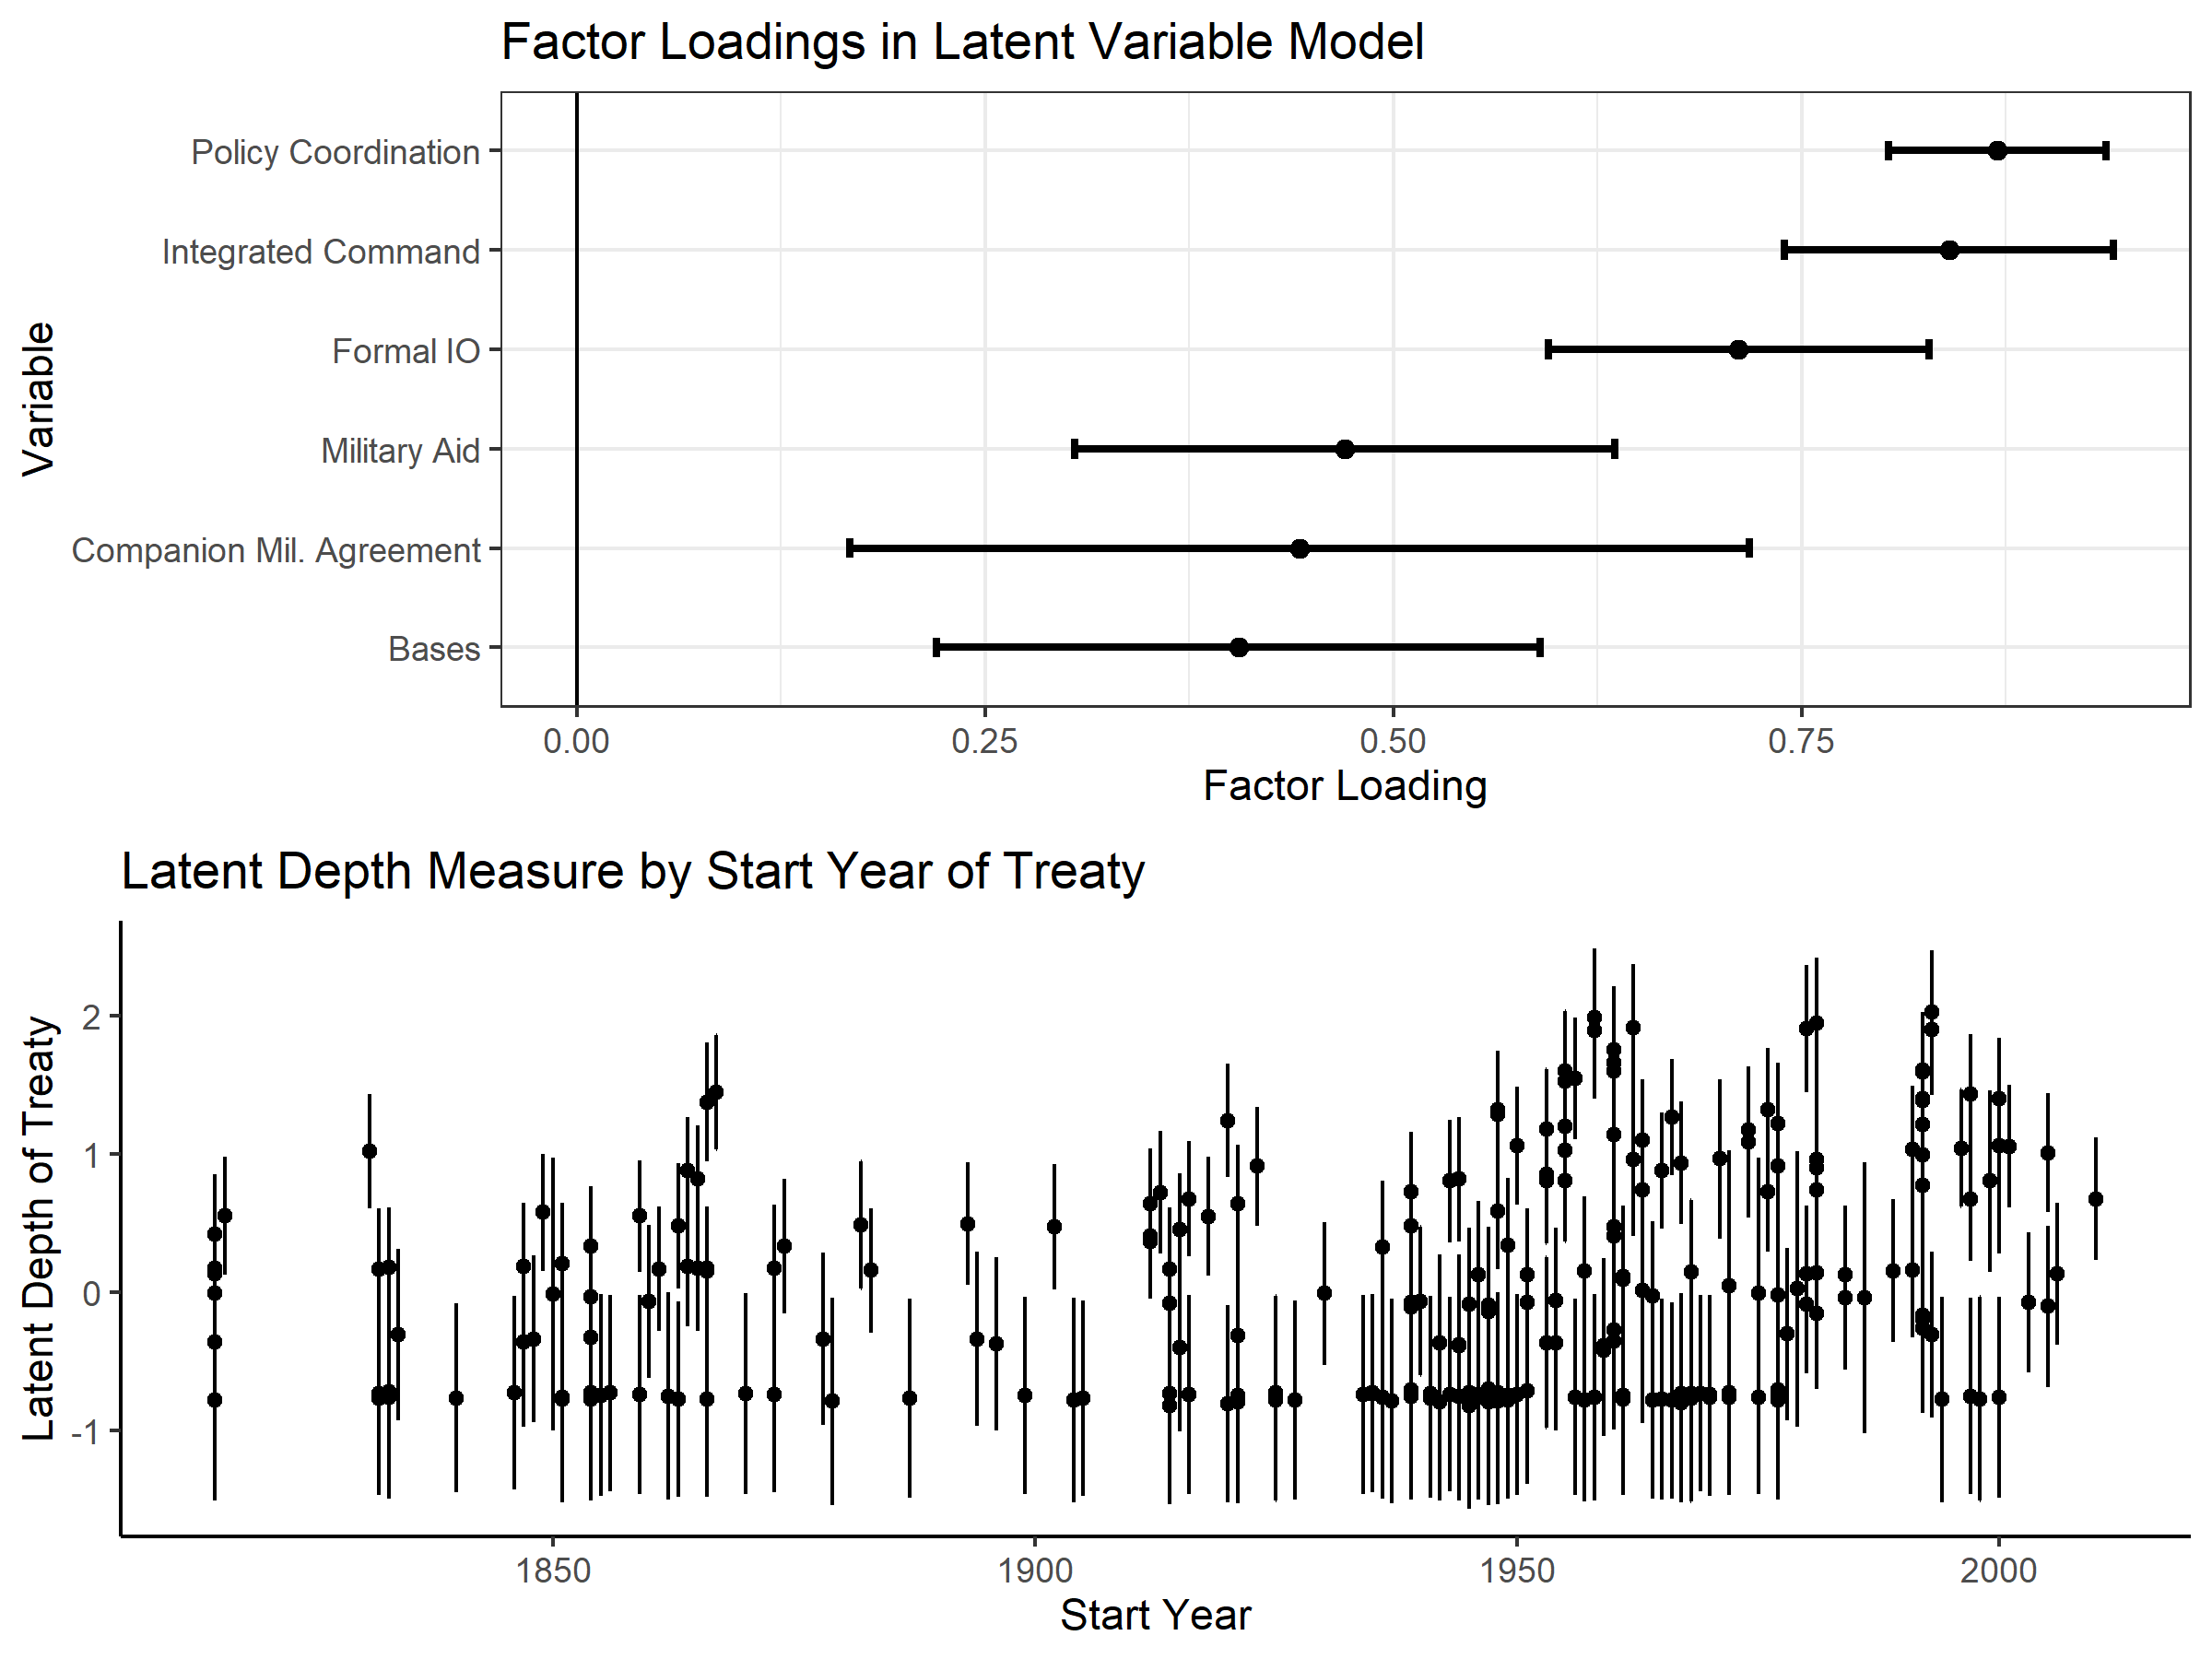
\includegraphics[width=0.95\textwidth]{../figures/loadings-measure.png}
\caption{Factor loadings and posterior distributions of the latent alliance treaty depth measure. Estimates from a semiparametic mixed factor analysis of offensive and defensive ATOP alliances from 1816 to 2016.}
\label{fig:loadings-measure}
\end{figure}


% discuss/justify the loadings
These factor loadings are sensible. 
Defense policy coordination, peacetime integrated command structures and formal organizations all draw alliance members into closer peacetime defense cooperation. 
The other variables do not require as much direct cooperation, with the potential exception of bases.
Although bases are costly, they also serve multiple functions and may not require as much direct cooperation. 
In addition to deterrence and increasing alliance credibility, states often use basing obligations to project power, so bases are used for other purposes besides promoting cooperation between allies, while the other factors provide for more direct cooperation.  


The measurement model predicts the treaty depth of each alliance using the factor loadings. 
The bottom panel of \autoref{fig:loadings-measure} summarizes the posterior distributions of the latent treaty depth measure for every alliance in the data. 
There is substantial variation in alliance treaty depth. 
Around half of all alliance treaties have some depth, and depth varies widely across alliances.
In the analysis, I measure treaty depth using the mean of the latent depth posterior for each alliance. 
The posterior mean captures the central tendency of latent treaty depth, and I show in the appendix that results are robust to accounting for uncertainty in the latent measure. 


The key independent variable is an ordinal indicator of electoral democracy in the most capable alliance member during the year of alliance formation. 
I use the the Lexical Index of Electoral Democracy (LIED) \citep{Skaaningetal2015} to measure electoral democracy.
This ordinal measure assesses the extent of electoral democracy in a country based on six components and ranges from zero to six.  
States with no elections of any kind have an index score of zero, while single-party elections receive score a one. 
Multiparty elections for legislature or executive roles that fall short of a minimum competition threshold score a two or three. 
States with minimally competitive multiparty elections for executive and legislative roles have an index score of four, and scores of five and six come from an expanded franchise.

I retain the full range of the electoral index of democracy for two reasons.\footnote{In the appendix, I report findings with a dummy indicator of full electoral democracy, which produces similar inferences.}
First, unlike some measures of democracy, the LIED scale isolates the key concept of my argument.
Furthermore, the order of the scale places competitive elections before full suffrage, in contrast to other measures of electoral democracy, which give participation and electoral institutions equal weight. 
Widespread participation is only meaningful if elections could remove the leader.


After measuring the lexical index for each country in an alliance, I identify the alliance leader.   
I code the alliance leader as the state with the largest composite index of national capabilities (CINC) score \citep{SingerCINC1988}, and measure their LIED score in the year the alliance formed.
The LIED of the most capable state therefore emphasizes the influence of the most capable alliance member and electoral democracy in that state.


I also measure executive constraints to examine whether it allows the opposition to check treaty depth. 
Furthermore, constraints are positively associated with electoral democracy.
I set an executive constraints dummy equal to one if the executive constraints concept in the Polity data codes a state as having executive parity or subordination to other branches of government.
In 85 of the 289 alliances the leader of the most capable state faces these constraints.



\subsection{Estimation Strategy}



I use several statistical models to estimate the association between democratic political institutions and treaty depth, including a two-stage hurdle model to account for selection into alliances. 
Modeling depth is complicated because the latent measure is skewed.
To facilitate model fitting, I rescaled latent depth to range between zero and one and modeled it with a beta distribution.
The flexibility of the beta distribution helps predict mean latent depth.\footnote{Using a beta distribution for the depth outcome also facilitates fitting models that account for uncertainty in the latent measure, which I include in the appendix. I also fit OLS and robust regression models of treaty depth without any rescaling, which lead to similar inferences. Results in the appendix.} 
The alliance leader democracy measures are the key independent variables in all these model specifications. 


In the regression models, I control for several correlates of treaty design and democratic institutions of the alliance leader. 
Key controls include dummy indicators of asymmetric alliances between non-major and major powers and symmetric alliances between major powers \citep{Mattes2012}\footnote{This leaves symmetric alliances between major powers as the base category for these two binary variables.} as well as the average threat among alliance members at the time of treaty formation \citep{LeedsSavun2007}. 
I also control for foreign policy similarity using the minimum value of Cohen's $\kappa$ in the alliance \citep{Hage2011}.
I draw on the ATOP data \citep{Leedsetal2002}, to adjust for for asymmetric treaty obligations, the number of alliance members and whether any alliance members were at war. 
To capture the role of issue linkages in facilitating alliance agreements and credible commitment \citep{Poast2012, Poast2013}, I include a dummy indicator of whether the alliance made any economic commitments. 
I also include an indicator of unconditional military support, which is correlated with democracy \citep{Chibaetal2015} and perhaps treaty depth. 
I adjust for a count of foreign policy concessions in the treaty, because concessions facilitate agreement in alliance negotiations \citep{Johnson2015}. 
Last, I account for the role of time and the international context by with a dummy indicator of alliance formation after 1945 and estimating the model in samples before and after 1945.\footnote{I also check whether findings about democracy are driven the United States. See the appendix for results with an additional control for U.S. membership, which are similar to the inferences below.}



\section{Results}


I find that electoral democracy in the most capable alliance member leads to deep alliance treaties. 
This pattern is apparent first in the raw data. 
Alliances where the leading alliance member had full electoral democracy were deeper on average, as the top panel of \autoref{fig:raw-data} shows. 
Many alliances with a democratic leader and treaty depth formed after 1945, but there are alliances before World War II that also fit this pattern. 

\begin{figure}[hbtp]
\centering
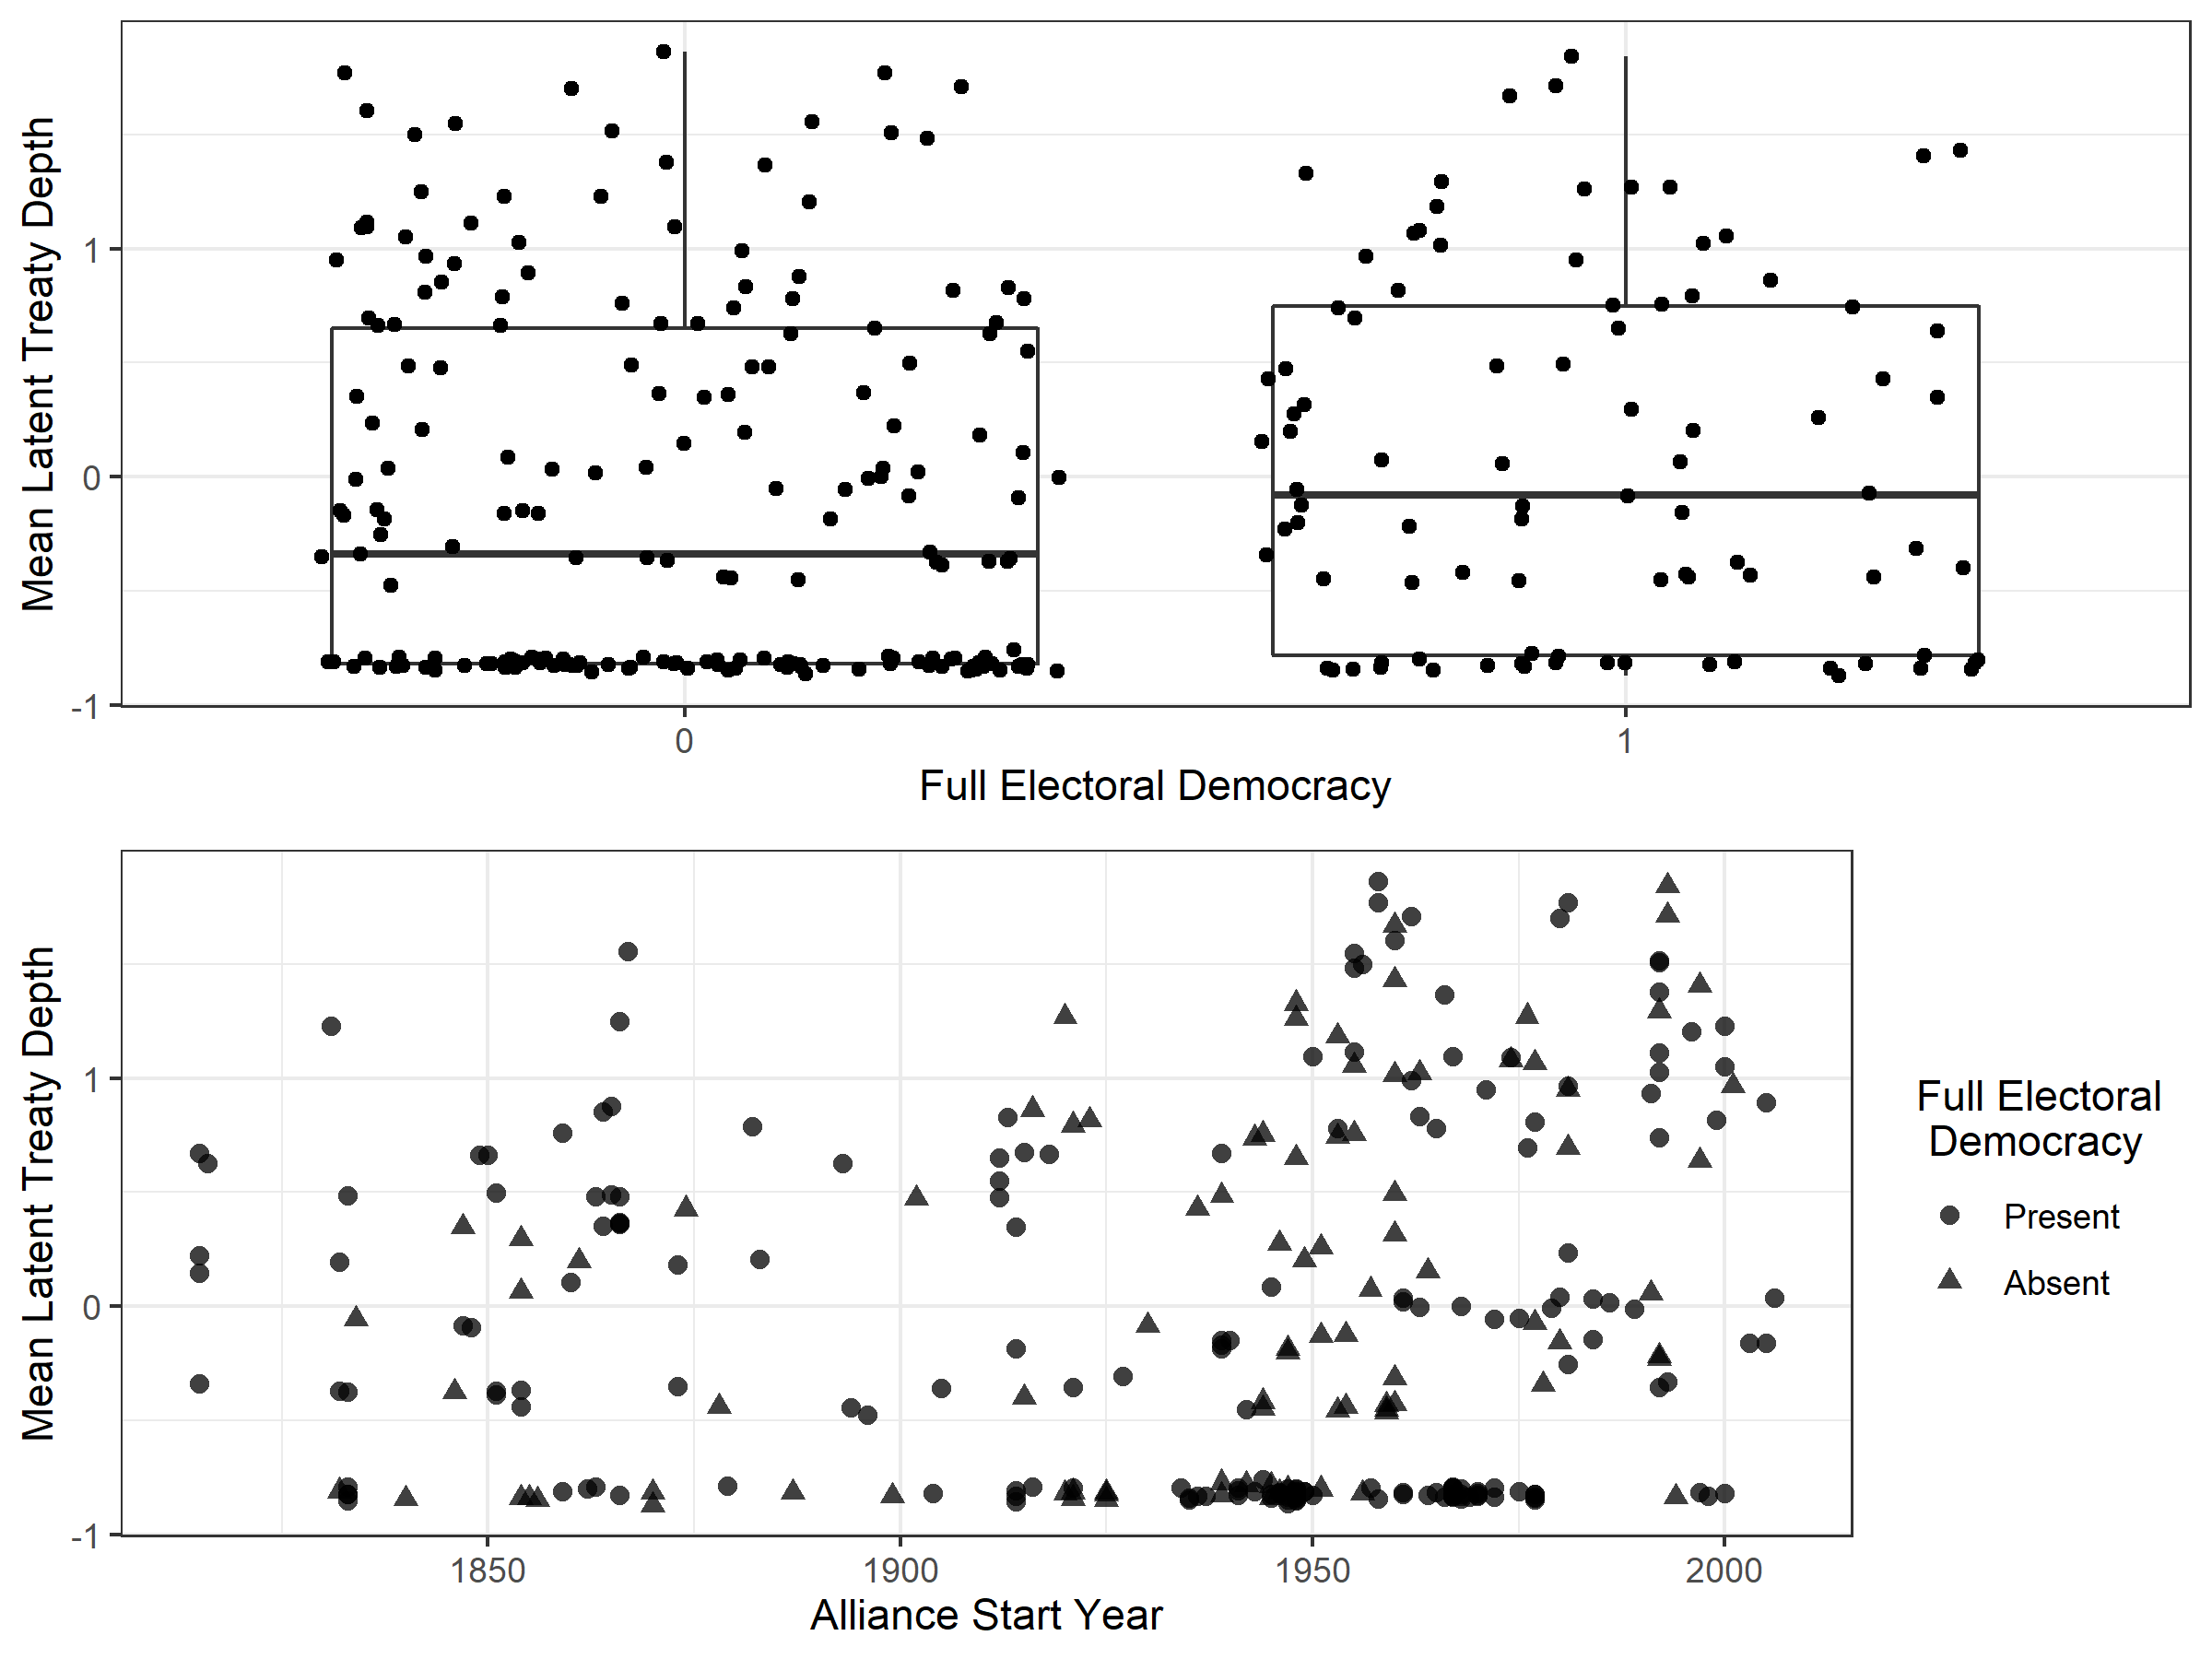
\includegraphics[width=0.95\textwidth]{../figures/raw-data.png}
\caption{Summary of raw data for alliance treaty depth and competitive elections. The top panel shows a boxplot with the distribution of mean latent treaty depth under alliances where the most capable member has high electoral democracy, and alliances where the leader does not have full electoral democracy. The bottom panel plots mean latent treaty depth over time, and marks alliances with full electoral democracy elections in the most capable state with triangular points. }
\label{fig:raw-data}
\end{figure}


The data in \autoref{fig:raw-data} does not adjust for potential confounding factors, however. 
\autoref{tab:reg-est} presents coefficient estimates from a series of beta regression models. 
In the first model, the most capable alliance member's polity score is the key independent variable. 
The second model divides democratic institutions into the lexical index of electoral democracy and executive constraints dummy.  
The third model estimates the same model on alliances before 1945. 
The final model estimates the association between electoral democracy, executive constraints, and treaty depth among alliances after 1945. 


These estimates are broadly consistent with the argument. 
More democratic institutions are positively correlated with treaty depth, per the alliance leader polity estimate in Model 1. 
Model 2 then suggests that this positive association is the result of electoral democracy, as increasing electoral democracy encourages alliance leaders to form deep alliances. 
Executive constraints has the opposite association with treaty depth. 
Although the electoral democracy coefficient is in the expected direction among alliances before 1945, the association is weaker and more uncertain.\footnote{The increased uncertainty is partially the result of a smaller sample.} 
Model 4 shows that the pattern of electoral democracy, executive constraints and treaty depth is more pronounced after 1945. 


\begin{table}[!htbp] \centering 
 \resizebox{.95\textwidth}{!}{
\begin{tabular}{@{\extracolsep{5pt}}lcccc} 
\\[-1.8ex]\hline 
\hline \\[-1.8ex] 
 & \multicolumn{4}{c}{\textit{Dependent variable:}} \\ 
\cline{2-5} 
\\[-1.8ex] & \multicolumn{4}{c}{Latent Depth (rescaled)} \\ 
\\[-1.8ex] & (1) & (2) & (3) & (4)\\ 
\hline \\[-1.8ex] 
 Alliance Leader Polity & 0.025$^{}$ &  &  &  \\ 
  & (0.004, 0.046) &  &  &  \\ 
  Lexical Index of Democracy &  & 0.209$^{}$ & 0.113 & 0.229$^{}$ \\ 
  &  & (0.115, 0.303) & ($-$0.065, 0.291) & (0.110, 0.348) \\ 
  Executive Constraints &  & $-$0.797$^{}$ & $-$0.416 & $-$0.987$^{}$ \\ 
  &  & ($-$1.241, $-$0.353) & ($-$1.137, 0.306) & ($-$1.635, $-$0.339) \\ 
  Economic Issue Linkage & $-$0.187 & $-$0.214 & 0.286 & $-$0.344 \\ 
  & ($-$0.510, 0.137) & ($-$0.533, 0.104) & ($-$0.175, 0.747) & ($-$0.781, 0.093) \\ 
  Unconditional Support & 0.439$^{}$ & 0.424$^{}$ & 0.064 & 0.516$^{}$ \\ 
  & (0.133, 0.746) & (0.120, 0.729) & ($-$0.450, 0.578) & (0.139, 0.893) \\ 
  Foreign Policy Concessions & $-$0.012 & $-$0.069 & 0.109 & $-$0.200$^{}$ \\ 
  & ($-$0.176, 0.153) & ($-$0.233, 0.094) & ($-$0.118, 0.336) & ($-$0.439, 0.038) \\ 
  Number of Members & 0.017 & 0.034$^{}$ & $-$0.012 & 0.068$^{}$ \\ 
  & ($-$0.010, 0.044) & (0.007, 0.061) & ($-$0.056, 0.031) & (0.030, 0.106) \\ 
  Wartime Alliance & $-$0.187 & $-$0.017 & $-$0.069 & $-$0.134 \\ 
  & ($-$0.566, 0.192) & ($-$0.394, 0.360) & ($-$0.468, 0.331) & ($-$1.117, 0.850) \\ 
  Asymmetric Obligations & 0.153 & 0.241 & 0.066 & 0.345 \\ 
  & ($-$0.194, 0.500) & ($-$0.104, 0.586) & ($-$0.335, 0.468) & ($-$0.252, 0.941) \\ 
  Asymmetric Capability & 0.393 & 0.333 & 0.558$^{}$ & 0.121 \\ 
  & ($-$0.077, 0.863) & ($-$0.134, 0.800) & (0.092, 1.024) & ($-$0.343, 0.586) \\ 
  Non-Major Only & 0.160 & 0.138 & 0.252 &  \\ 
  & ($-$0.358, 0.677) & ($-$0.376, 0.651) & ($-$0.330, 0.834) &  \\ 
  Average Threat & 0.874$^{}$ & 0.965$^{}$ & 1.643$^{}$ & 0.653 \\ 
  & (0.038, 1.710) & (0.132, 1.798) & (0.419, 2.867) & ($-$0.487, 1.793) \\ 
  Foreign Policy Disagreement & 0.295 & 0.215 & 0.440 & 0.043 \\ 
  & ($-$0.186, 0.775) & ($-$0.256, 0.686) & ($-$0.163, 1.044) & ($-$0.712, 0.798) \\ 
  Post 1945 & 0.208 & 0.196 &  &  \\ 
  & ($-$0.169, 0.584) & ($-$0.175, 0.566) &  &  \\ 
  Constant & $-$1.658$^{}$ & $-$1.956$^{}$ & $-$2.536$^{}$ & $-$1.347$^{}$ \\ 
  & ($-$2.399, $-$0.916) & ($-$2.741, $-$1.170) & ($-$3.511, $-$1.562) & ($-$2.374, $-$0.320) \\ 
 \hline \\[-1.8ex] 
Observations & 276 & 276 & 118 & 158 \\ 
Log Likelihood & 56.692 & 63.188 & 44.319 & 35.603 \\ 
\hline 
\hline \\[-1.8ex] 
\textit{Note:}  & \multicolumn{4}{r}{95\% Confidence Intervals in Parentheses.} \\ 
\end{tabular} 
}
  \caption{Beta regression estimates of the association between alliance leader democracy and treaty depth from 1816 to 2012.} 
  \label{tab:reg-est} 
\end{table} 


Inferences about the control variables are also interesting.
More alliance members and asymmetric capability both increase depth, as does external threat.
The association between threat and depth is stronger before World War II, while multilateral alliances after 1945 have more depth. 
Unconditional military support and treaty depth are positively correlated, especially after 1945. 


To assess the substantive impact of elections, I estimated the marginal effect of electoral democracy. 
In the scenarios, I held all other variables at their mode or median, varied the lexical index of electoral democracy across its full range and altered the presence or absence of electoral constraints. 
\autoref{fig:results-depth} plots the estimated marginal effect of electoral democracy across 14 combinations of executive constraints and electoral democracy, holding all else equal. 


\begin{figure}[hbtp]
\centering
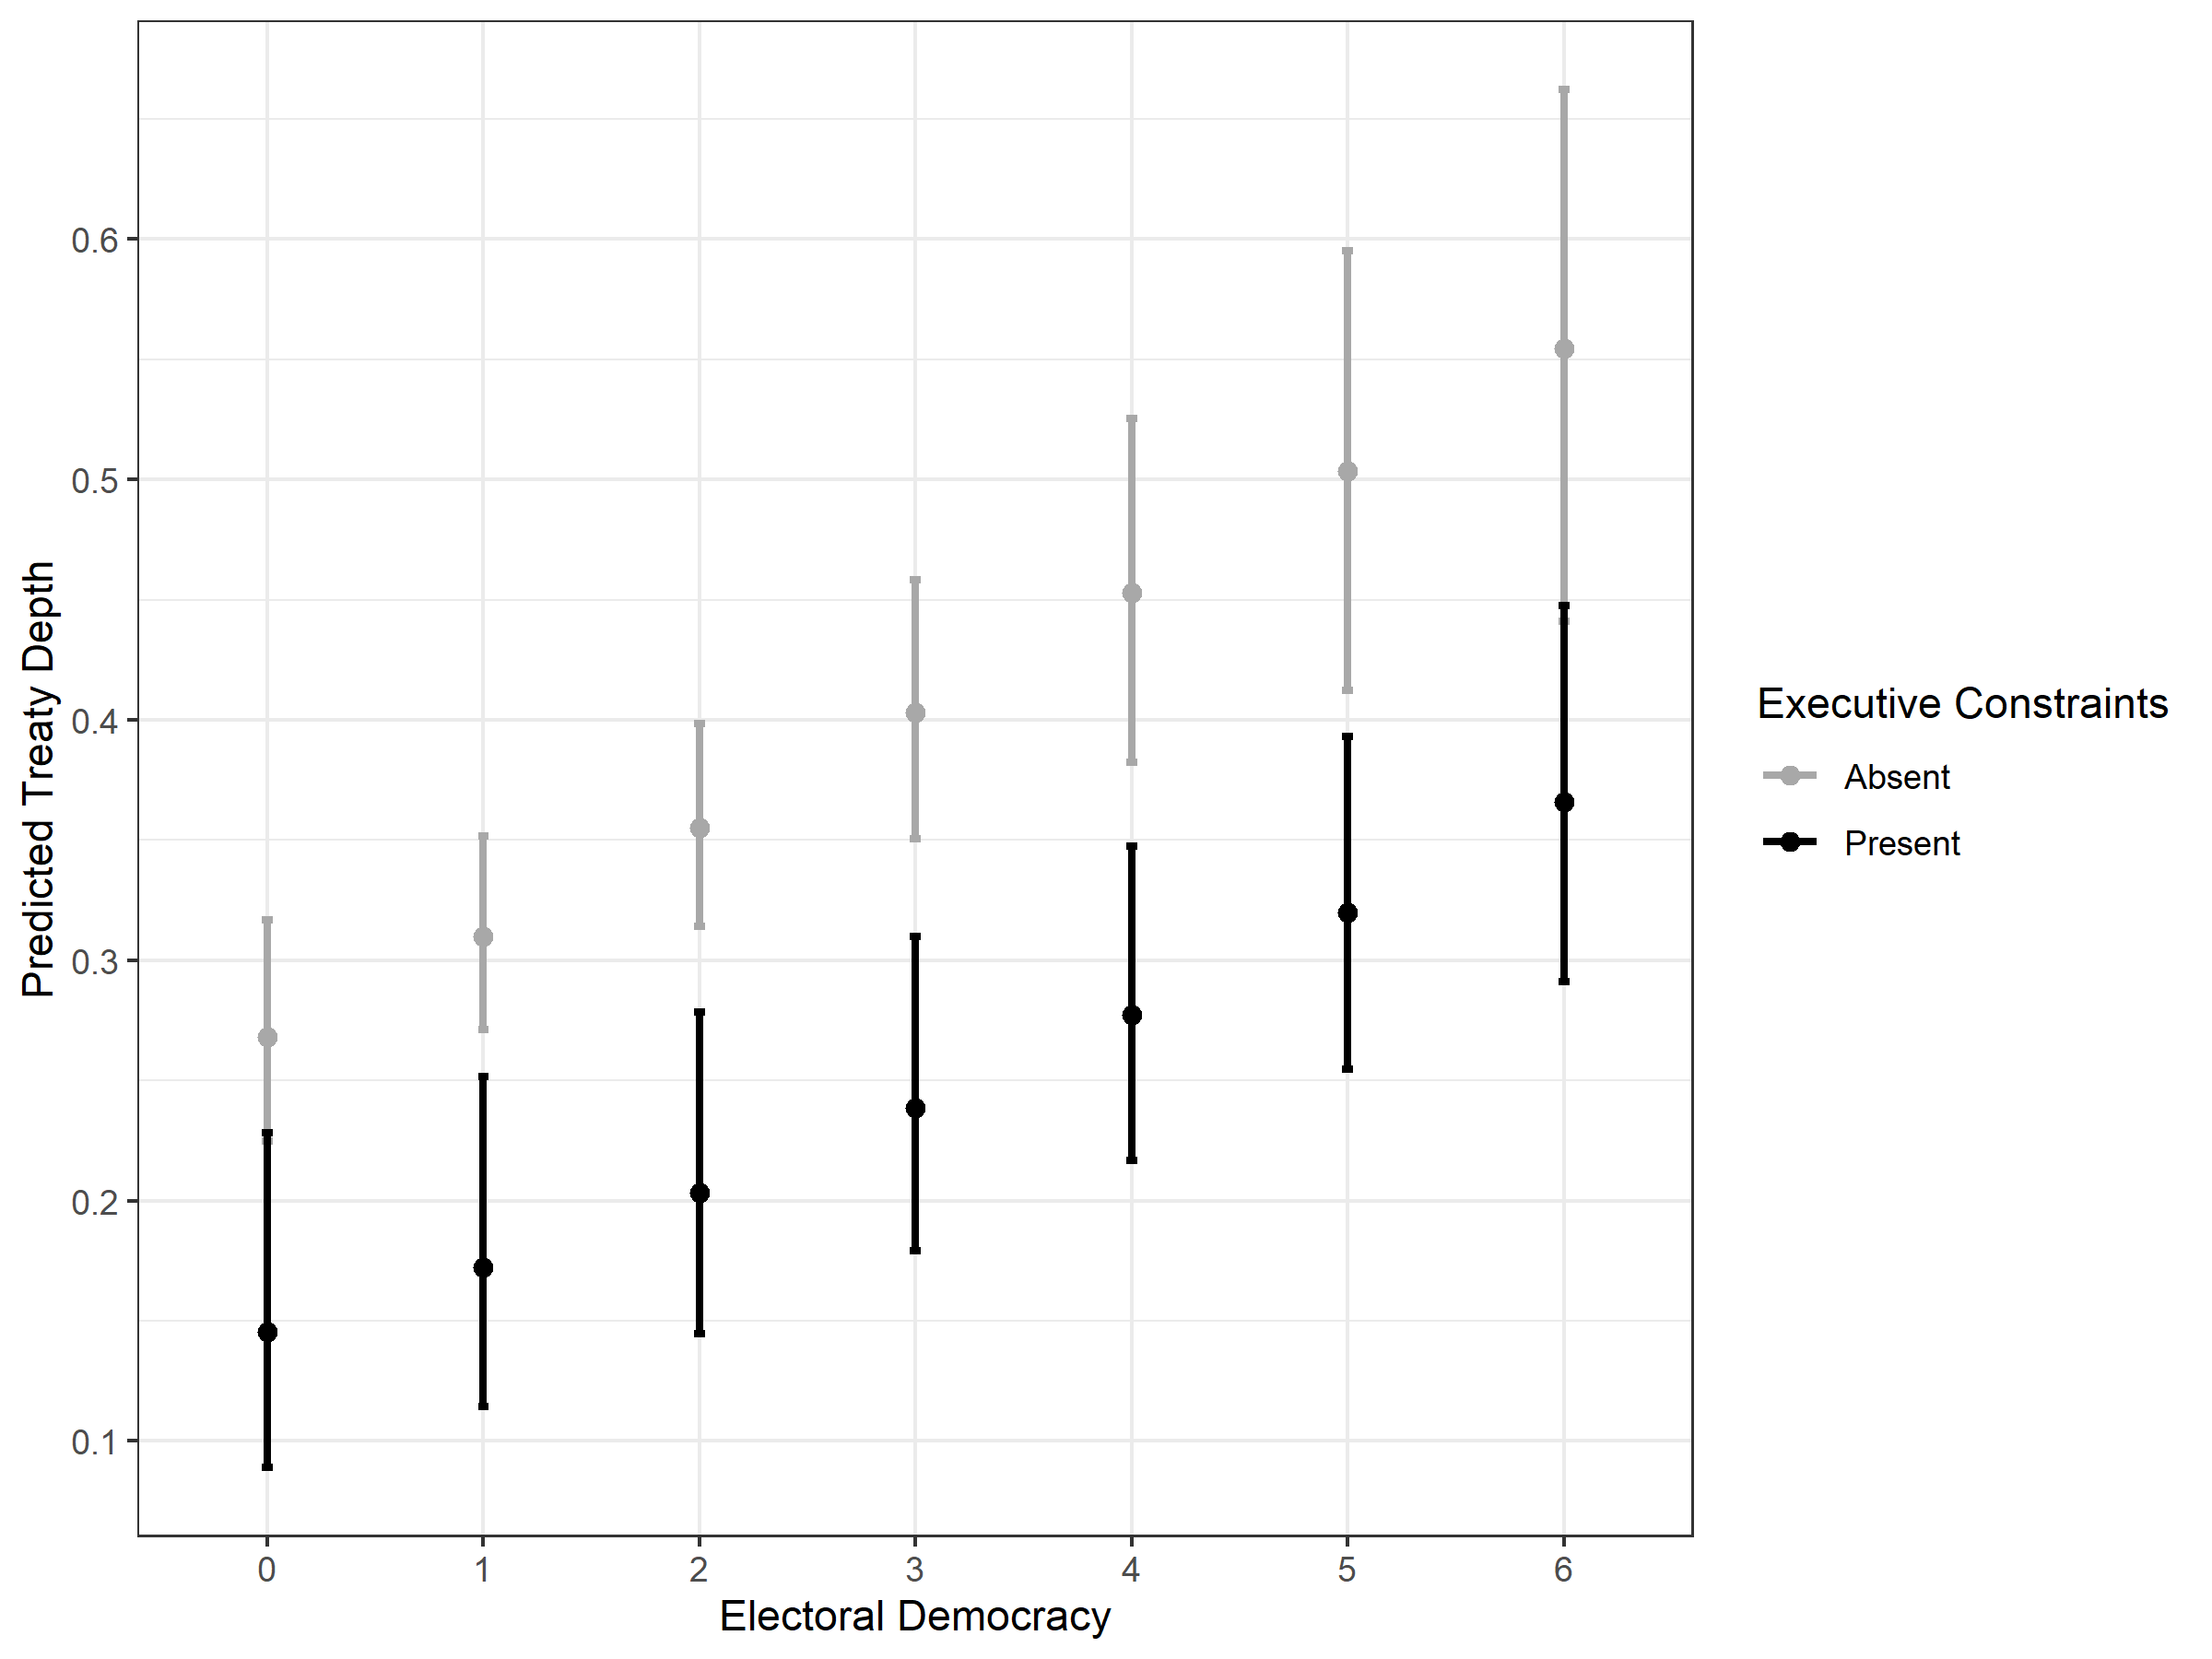
\includegraphics[width=0.95\textwidth]{../figures/results-depth.png}
\caption{Predicted treaty depth across different combinations of electoral democracy and executive constraints. Each scenario plots predicts treaty depth at a level of the lexical index of electoral democracy, with executive constraints present or absent. All other variables held at their mean or median.}
\label{fig:results-depth}
\end{figure}


Electoral democracy has a clear substantive impact on alliance treaty depth.
Predicted depth given full electoral democracy in the alliance leader ranges between .29 and .45 more latent depth when executive constraints are also present.
I focus on this estimate because most states with full electoral democracy also have executive constraints. 
As rescaled depth ranges between zero and one, these are large substantive effects.


\autoref{fig:results-depth} shows that greater electoral democracy increases treaty depth. 
Executive constraints attenuate this relationship, but do not eliminate the positive association between electoral democracy on alliance treaty depth. 
In the following, I consider the role of prior changes in the ruling coalition. 


\subsection{Electoral Democracy and Coalition Changes}


First, I use information on the connection between electoral democracy and changes in the coalitions backing a leader to differentiate the lock in process from a pure audience costs argument.
Part of my argument claims that electoral democracy increases the likelihood of leadership transitions that empower a new coalition. 
Therefore, electoral democracy and prior changes in the source of leader support should be positively correlated.
Using the Changes in the Sources of Leader Support (CHISOLS) data \citep{Mattesetal2016}, I find that this is the case. 
Decades with more years of democracy have more frequent changes in the ruling coalition. 
In particular, Alliance leader electoral democracy is positively correlated with the number of leadership changes that brought a new coalition to power during five and ten year windows prior to alliance formation. 


Furthermore, the number of ruling coalition changes in the most capable state before alliance formation is positively correlated with treaty depth. 
This inference is based on modified beta regression models where I replaced the lexical index of electoral democracy with the number of changes in the sources of leader support in the five and 10 years before alliance formation. 
\autoref{fig:ch-plot} plots the key coefficient estimates from these revised models, which use both raw and logged ruling coalition changes.\footnote{Due to limits in the coverage of the CHISOLS data, this analysis covers from 1920 to 2006.}
The positive association between prior ruling coalition changes and treaty depth holds across two temporal windows and logged or raw counts of coalition changes.


\begin{figure}[hbtp]
\centering
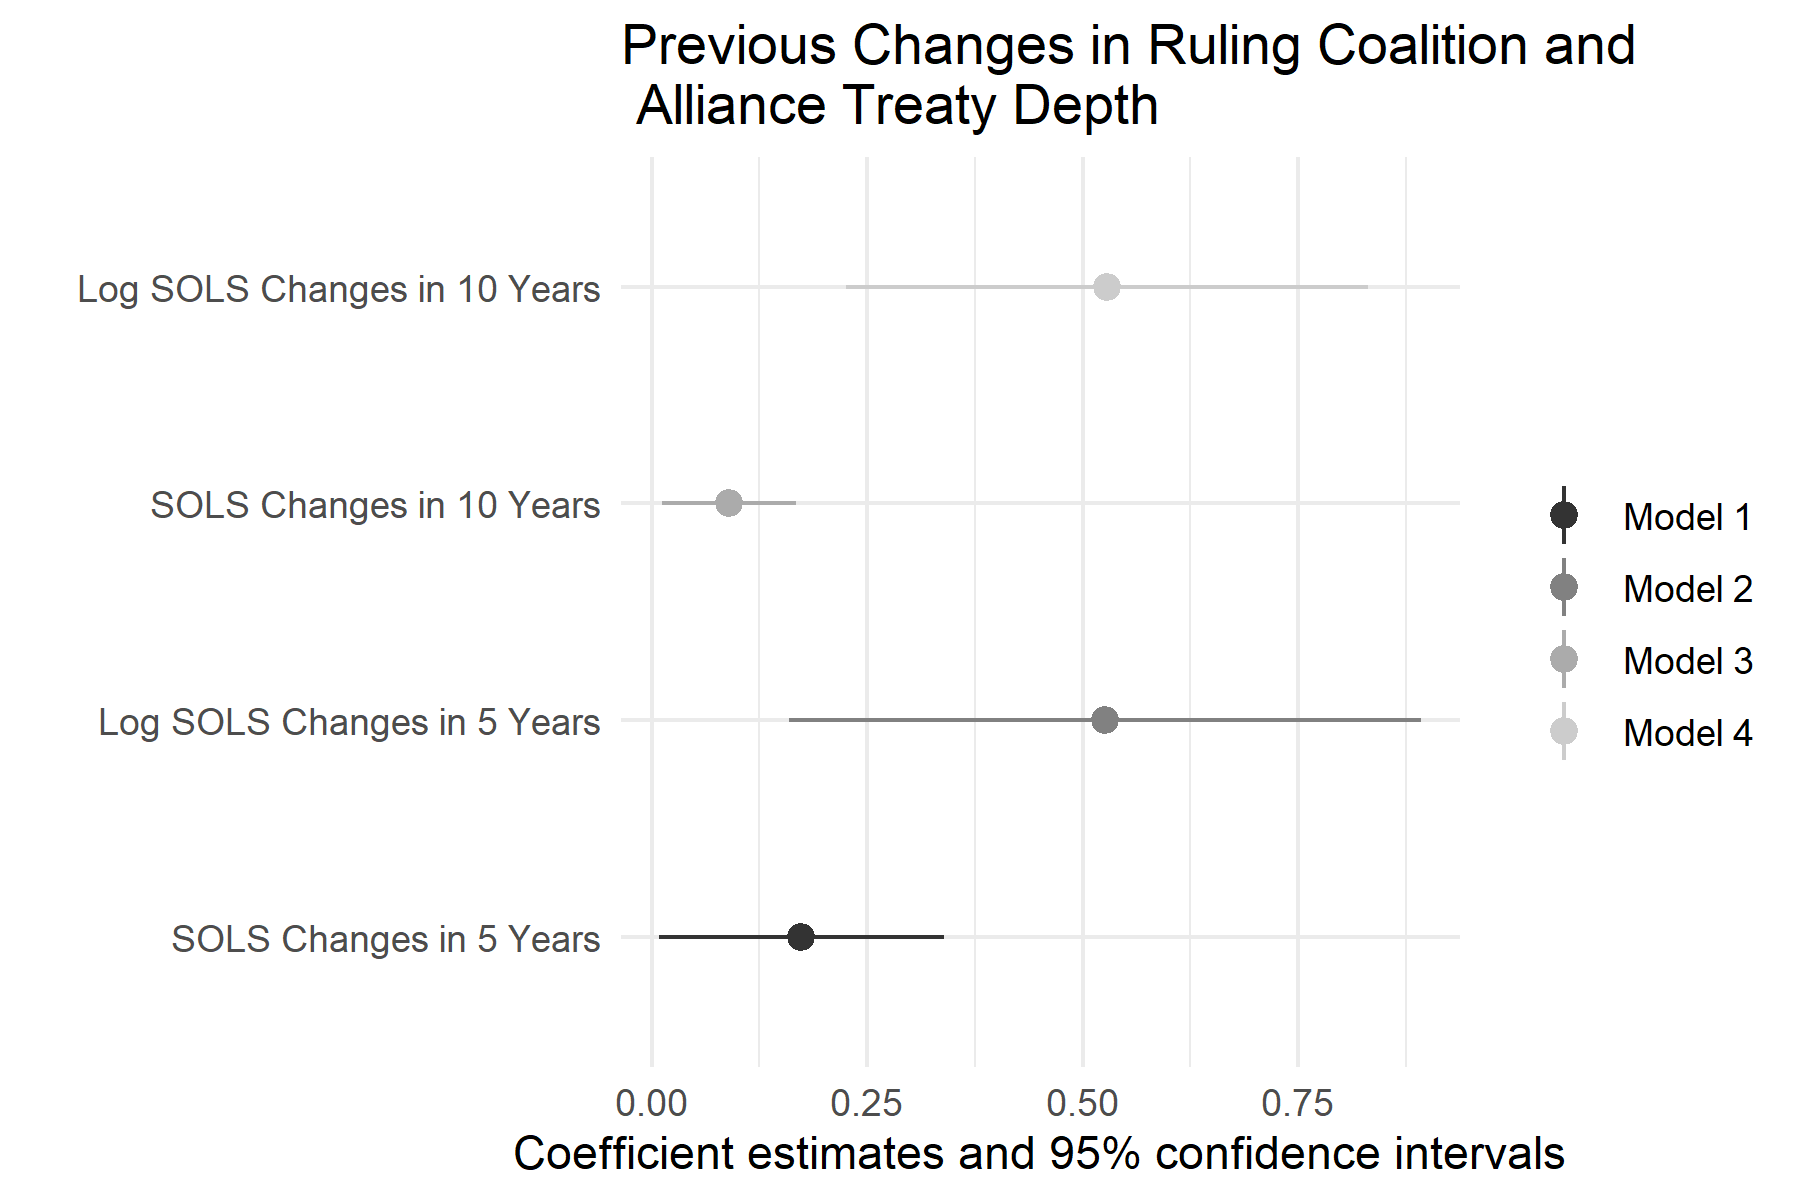
\includegraphics[width=0.95\textwidth]{../figures/ch-plot.png}
\caption{Estimated association between prior changes in the sources of leader support in the most capable alliance member and alliance treaty depth. Estimates based on beta regression models of rescaled treaty depth from 1920 to 2006. One model uses the number of ruling coalition changes in the five years before alliance formation, while the other uses the same measure from the decade before alliance formation.}
\label{fig:ch-plot}
\end{figure}


The estimates in \autoref{fig:ch-plot} are consistent with the claim that depth helps lock in alliance commitments in the face of democratic leadership turnover.
They are less consistent with a pure audience costs argument, which would not predict a positive relationship between prior leadership change and depth.   
Thus, leadership turnover concerns in democracies are a salient driver of treaty depth. 
 

Another implication of the argument is that a selection process is present. 
Observed treaty depth reflects situations where leaders can secure voter approval of alliance formation.
In the next section, I check the robustness of the electoral democracy results by accounting for non-random selection into alliances. 


\subsection{Hurdle Model of Treaty Depth} 


In this section, I account for non-random alliance formation by fitting a hurdle model to data that combines a stratified random sample of non-allied groups of states with observed alliances. 
This research design produces similar inferences: electoral democracy in the most capable alliance member increases treaty depth. 
I also find a weaker association between executive constraints and treaty depth. 


My research design for this robustness check follows established procedures for dealing with selection into alliances and treaty design. 
I followed the suggestions of \citet{Poast2010} for k-adic data, because some alliances have more than two members. 
First I constructed a random sample of groups of states that could have formed an alliance in each year, but did not \citep{FordhamPoast2014}.
Then I took a stratified sample of the non-allied k-ads to include five times as many non-allied observations as alliance observations for each observed value of alliance size. 
For example, there are 215 bilateral alliances, so I sampled 1075 non-allied bilateral groups. 
There is only one alliance with 34 members, so I added five non-alled k-ads with 34 members. 
Finally, I summarized key characteristics of these non-allied k-ads, including average Polity score, the electoral democracy of the most capable member, the number of members, mean threat, asymmetric capability, and wartime, and merged the non-allied data with the observed alliance data. 


To model alliance treaty alliance design, I emulated the research design of \citet{Chibaetal2015}, who estimated a hurdle model to assess whether democracies were more likely to offer conditional obligations.
Hurdle models have two stages or parts which account for non-random selection into alliances.
A first stage model predicts which observations clear the hurdle to a second stage with non-zero outcome values. 
Observed alliances are the set of observations that cleared the hurdle and have an alliance treaty. 
Unlike a sample selection model, the second stage in a hurdle model is logically undefined, which is how alliance treaty design works.\footnote{Hurdle models also do not require an exclusion restriction for identification.} 
Unless states overcome the barriers to alliance formation, no agreed treaty content exists. 


Because I examine a continuous measure of latent depth, I estimate a Bayesian gamma hurdle model using the BRMS package for \textsf{R}, which employs STAN for fully Bayesian inference \citep{Buerkner2017}.
To have zero values for the outcome at the hurdle stage and positive values for the gamma-distributed outcome, I adjusted the scale of the latent depth measure by adding one, which shifted the distribution onto uniformly positive values. 
K-ads without an observed alliance then had a depth score of zero. 


In both models, I use average democracy, alliance leader executive constraints and electoral democracy, mean threat, asymmetric capability, wartime, group size and year varying intercepts to predict whether each group of states clears the alliance formation hurdle.
In the second stage, electoral competition and executive constraints in the most capable alliance member, the number of members, mean threat, dummy indicators of asymmetric capability wartime and year varying intercepts model treaty depth in observed alliances. 


After accounting for non-random alliance formation with the hurdle model, I find partially similar results about democratic institutions. 
\autoref{fig:results-hurdle} plots predictions from the hurdle model estimates across the range of the two democratic institution measures. 
This figure shows the predicted marginal effect of electoral democracy and executive constraints in the alliance leader on shifted treaty depth, along with 95\% credible intervals.
Electoral democracy in the most capable alliance member increases treaty depth, but the effect of executive constraints is weaker than the single-equation results.  


\begin{figure}
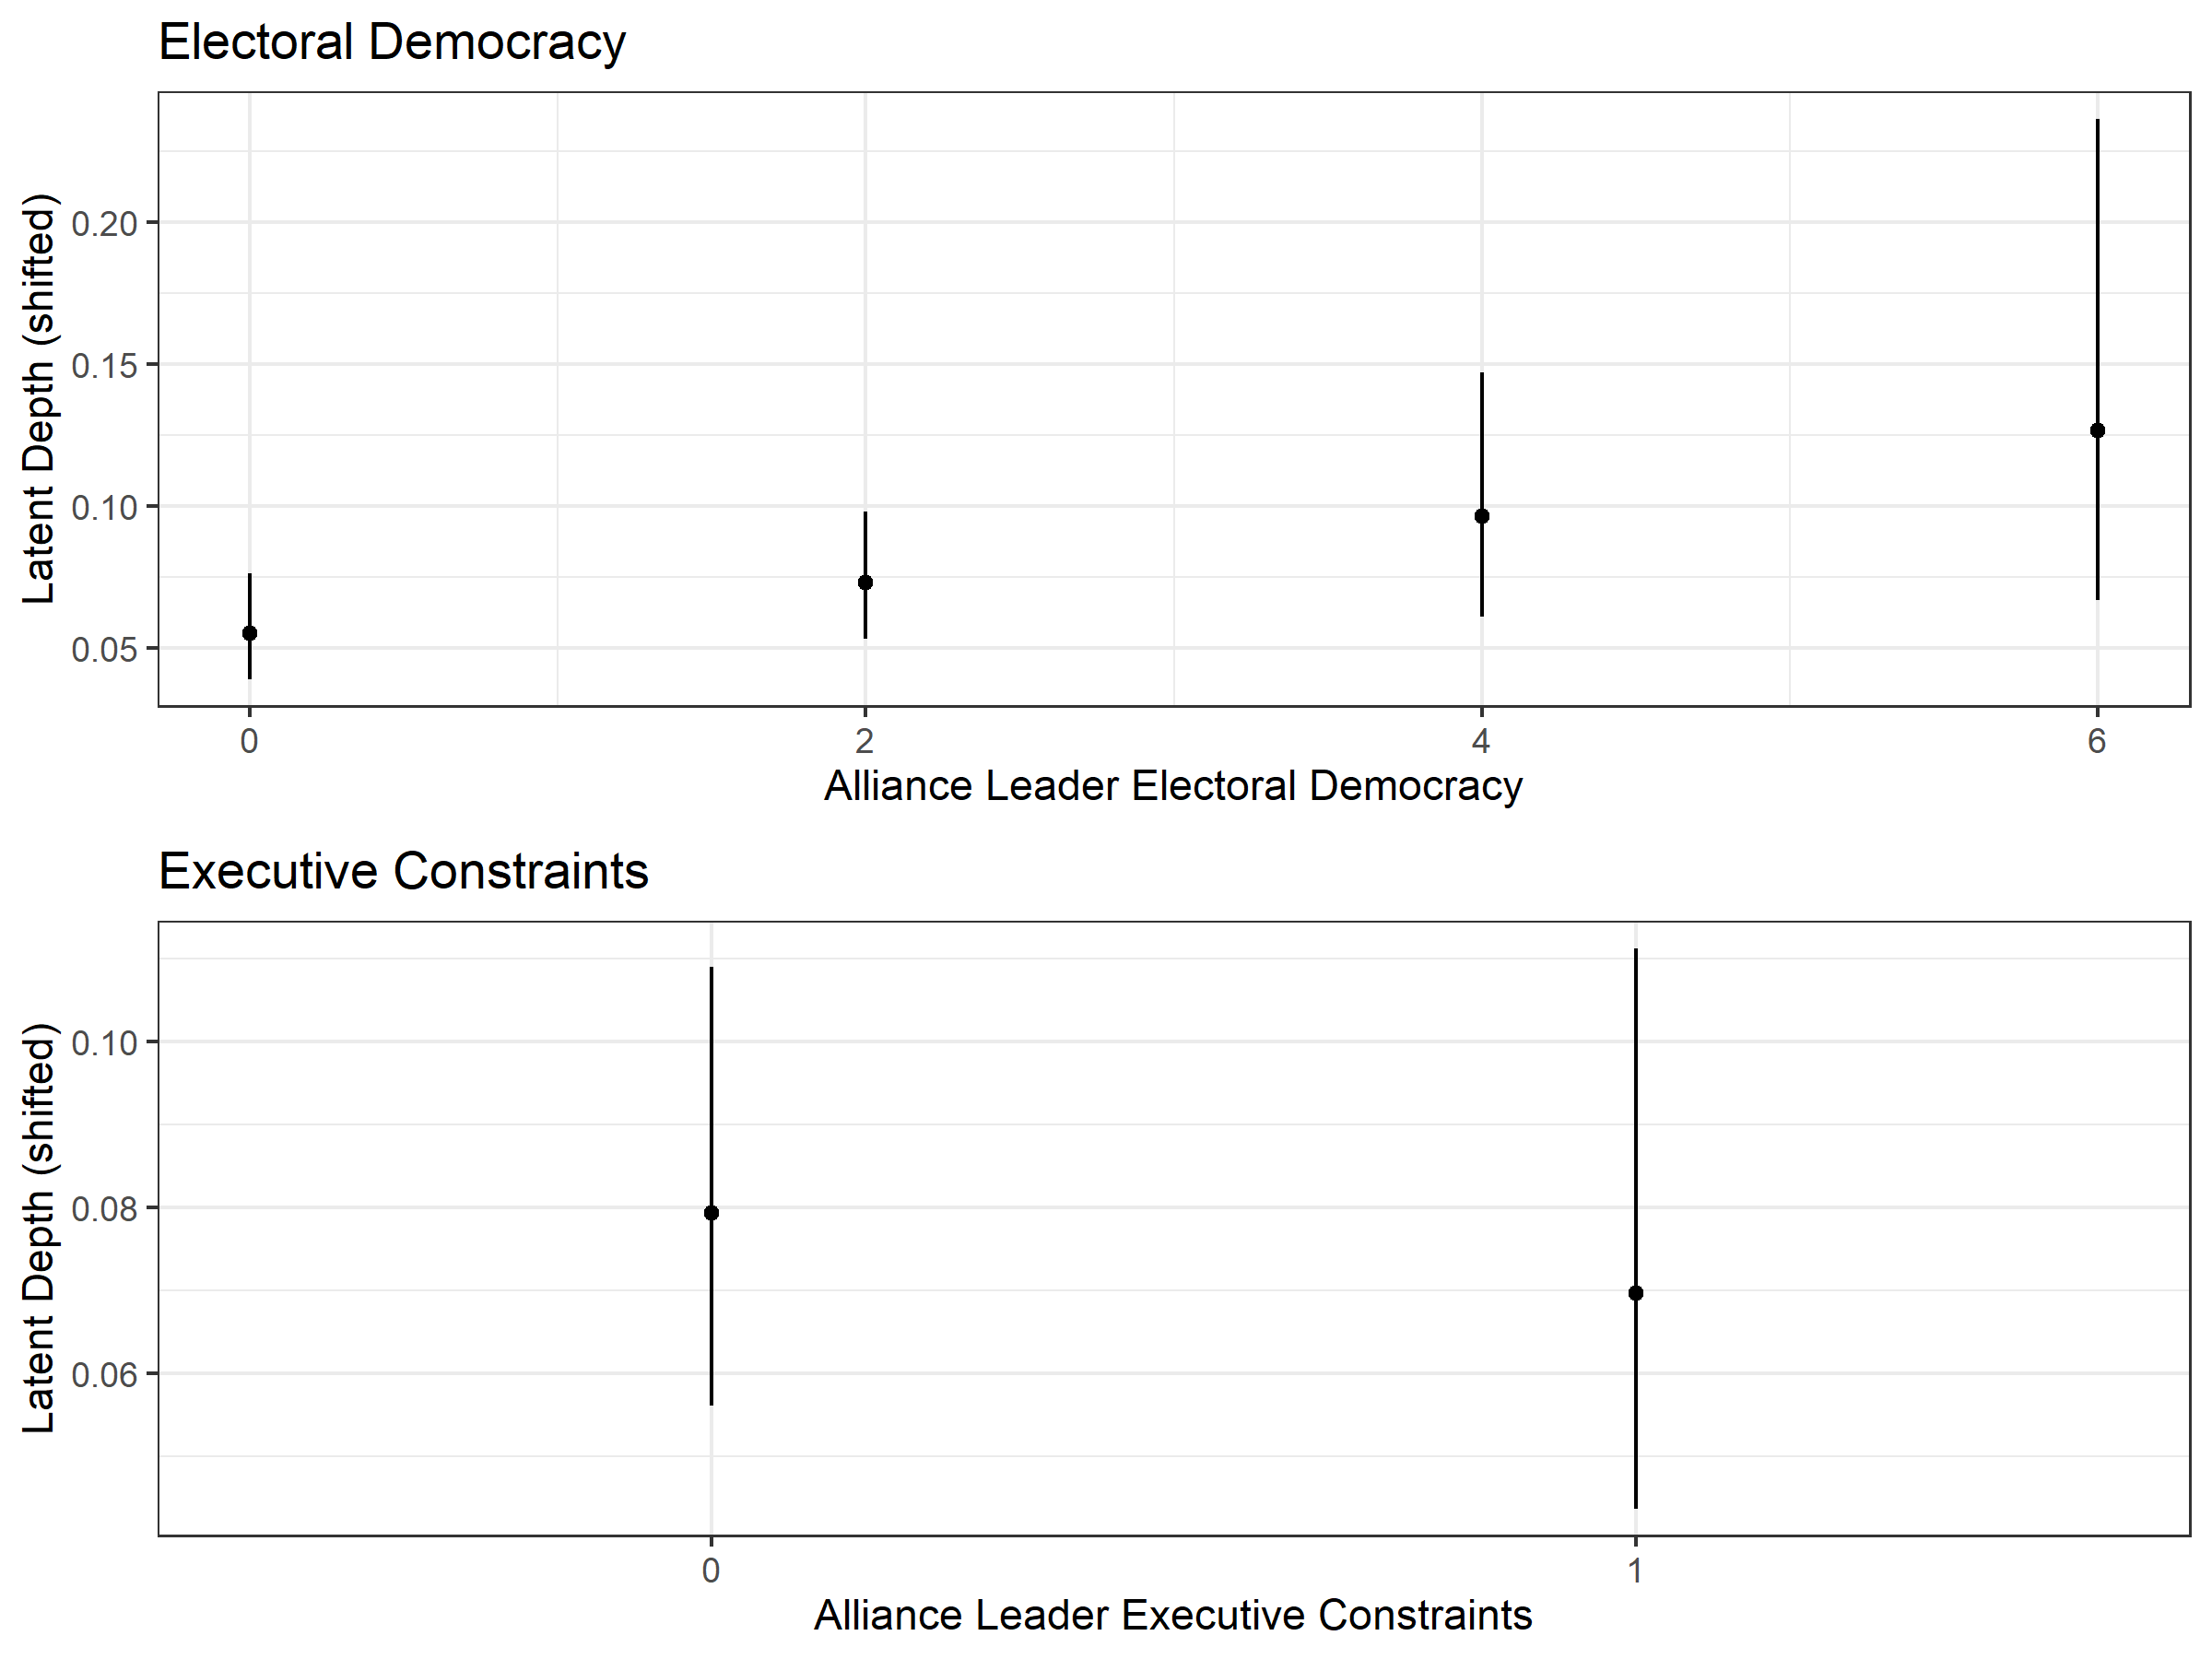
\includegraphics[width=.95\textwidth]{../figures/results-hurdle.png}  
\caption{Predicted treaty depth by electoral democracy and executive constraints in the most capable alliance member when the treaty formed. Estimates are based on a hurdle model of alliance treaty depth. The line marks predicted values, and the shaded areas encapsulate the 95\% credible interval. Predictions hold all other variables constant.}
\label{fig:results-hurdle}
\end{figure}


Even after considering non-random alliance formation, electoral democracy encourages deep alliances. 
When democratic leaders can form an alliance, they often buttress the treaty against leadership turnover through depth. 
After accounting for non-random selection into alliances, executive constraints are not associated with shallower alliances.
This implies that when the opposition cannot or does not check alliance formation, they have limited influence over treaty depth. 


Democratic political institutions shape alliance treaty design. 
Electoral democracy pushes alliance leaders to form deep alliances. 
After accounting for non-random selection into observed alliances, executive constraints do not reduce treaty depth. 
To further illustrate the theoretical process, I now examine the North Atlantic Treaty Organization (NATO).



\subsection{NATO Treaty Design}


I use NATO to show the theoretical mechanisms for two reasons. 
First, the process behind NATO applies to multiple alliances, as other US alliance treaties have similar designs. 
Second, NATO is the most important alliance in international politics, as it has a crucial role in the structure of international relations by connecting the United States and Europe. 
Because NATO is an exceptionally durable and consequential alliance, understanding how its treaty design is worthwhile. 
In this brief discussion, I do not offer a comprehensive picture of NATO negotiations.\footnote{See \citet{Kaplan2007} and \citet{Poast2019a} for useful overviews.} 
Instead, I highlight the rationale behind alliance treaty depth in NATO, which includes the Atlantic Council and basing rights. 


After World War II, the United States sought to protect Europe from the USSR. 
Although the United States and Europe both perceived a serious threat, establishing a credible promise of military intervention was difficult. 
The United States had to overcome European fears of transient commitment.
\citet[pg. 14]{Sayle2019} highlights the importance of U.S. domestic political change by noting that, ``the future allies of the United States knew how easily presidents, and their commitments, could change. They wanted an agreement that would survive the transition from one president to the next.'' 


To increase the credibility and perceived durability of NATO, the United States used treaty depth.  
A 1949 State Department telegram explicitly connected costly cooperation and reassurance, by noting the view of two ambassadors that ``Delay in the aid program would resurrect doubts as to the dependability and consistency of US policy'' \citep{state-summary-0607-49}. 
A 1951 presentation by Dean Acheson to Dwight Eisenhower argued that European allies ``fear the inconstancy of United States purpose in Europe. ... These European fears and apprehensions can only be overcome if we move forward with determination and if we make the necessary full and active contribution in terms of both military forces and economic aid'' \citep[pg. 3]{Acheson1951}. 


To start, the United States supported the Atlantic Council, an international organization and the main source of depth in the NATO treaty. 
The United States used the Atlantic Council to coordinate collective defense and increase the perceived reliability of the alliance. 
Investing in the Atlantic Council and related joint military planning helped assuage European fears. 
For example, U.S. officials thought that the British Foreign Minister viewed a U.S. supreme commander in Europe as ``a stimulus to European action'' in NATO \citep{Acheson1950}. 
The ``organization and integrated military command ... helped alleviate European concerns about the less-than-rock-solid article 5'' \citep[pg. 26]{Sayle2019}.


% evidence of turnover concerns here
NATO also added formal approval of basing rights for U.S in a 1951 additional protocol.  
Bilateral agreements on troop deployments thus became another instrument of reassurance. 
In 1950 the Germans formally requested clarification on whether an attack on US forces in Germany would be treated as an armed attack on the United States- and US policymakers said that it would \citep[pg. 395]{Acheson1969}.  
Many European members saw troop deployments as a guarantor of stable U.S. commitment. 
U.S. bases also assured other allies that German militarism would not threaten Europe. 
Even after World War II, a continued U.S. presence in Europe was not a given, as many Congressmen pushed for U.S. troops to leave Europe, and the United States regularly stated aspirations that Europeans would eventually provide all of their security \citep[pg. 20]{Sayle2019}. 

% leave out discussion of positive sell for now
%There is also evidence that U.S. leaders thought depth could help ``sell'' NATO to the public. 
%Policymakers justified NATO participation in part by arguing that it would facilitate more efficient defense spending. 
%In an interview with NBC on March 29, Ambassador at Large Philip Jessup argued that ``One defense program is cheaper and more effective than a dozen national programs. It entails the pooling of information, a joint defense strategy and a pooling of military resources for defense.''
%This claim sought to assuage concerns that NATO would reduce the ``peace dividend'' after World War II. 


% Sum up 
In NATO, allied concerns with leadership change encouraged deep military cooperation, which reassured European allies of U.S. commitment. 
This suggests that the theoretical mechanisms are plausible. 
In the next section, I summarize some implications of the results from this case discussion and the statistical models and offer concluding thoughts. 



\section{Discussion and Conclusion} 


% main evidence summary
The statistical models generate consistent evidence for the depth and electoral democracy hypothesis, and the NATO illustration suggests that the theoretical mechanisms are plausible. 
Electoral democracy is positively correlated with treaty depth across several models, including one that accounts for selection into alliances. 
This reflects efforts to limit the impact of leadership changes on alliance credibility. 


% limitations
The above argument and evidence have two limitations.
First, I only examine variation in formal treaty design. 
This omits treaty implementation, which can diverge from the formal commitment.   
Formal treaty depth often reflects practical depth, but it may understate some differences between alliances. 
Changes in realized alliance depth are a useful subject for future inquiry, but will require extensive data collection.
Second, I examine 280 alliances, so the sample size is limited. 
Inferences from small samples can be more sensitive to model and data changes. 


Shortcomings aside, this paper has three implications for scholarship. 
First, alliance treaty design is often driven by domestic political considerations as well as international politics. 
Attempts to ensure commitment by successors who represent different coalitions encourages democratic leaders to design deep alliance treaties. 

Second, democracies do not make fully limited alliance commitments.
Even if democracies impose conditions on military support, treaty depth adds costly obligations.
As a result, democracies make robust alliance commitments in one way, and limited commitments in another. 


Last, some of the lessons from this work might apply to the design on international institutions in general \citep{DownesRocke1995, MartinSimmons1998, Koremenosetal2001, Thompson2010}.
In the same way that democracies use depth to support allies while managing electoral politics, democracies may undertake deep international commitments in other ways. 
The same mix of limited core obligations and deep cooperation may characterize other international institutions with democratic leadership. 


The findings raise several questions for future research.  
For one, they address debates about whether democracies make more credible commitments. 
The net effect of democracy on alliance credibility includes conditions on military support, treaty depth, and the direct effect of democratic institutions and domestic politics. 
These three mechanisms may have competing or conditional effects, which could explain mixed findings about the credibility of democratic commitments \citep{Schultz1999, Leeds1999, Thyne2012, DownesSechser2012, PotterBaum2014}.
Future research should combine the components of democracy and democratic alliances to asses the net effect of democracy on credible commitment in international relations. 


Scholars should also consider how alliance treaty design varies across different types of autocracies. 
The extent and sources of political competition in autocracies varies widely. 
Differences in who selects leaders and what information those actors have about foreign policy \citep{Weeks2008} may help explain alliance treaty design.
For example, personalist leaders with few public or elite constraints on their foreign policy may design alliances with depth and unconditional military support. 
Single party states where leaders face an informed elite may prefer fully limited commitments with shallow and conditional obligations. 


Furthermore, scholars might consider how different aspects of alliance treaty design are related \citep{FjelstulReiter2019}. 
As states attempt to make credible alliance commitments, they employ a variety of treaty obligations. 
Scholars should examine how conditions on support, depth and issue linkages are related in alliance treaty design. 


In conclusion, electoral democracy encourages democracies to use treaty depth to increase the credibility of their alliances. 
Deep alliances reassure democracies' alliance partners in the face of potential leadership turnover. 
By shaping leaders' path to and from office, domestic political institutions influence how states make credible and durable alliance treaties.




 
\bibliography{../../../MasterBibliography} 





\end{document}
